\documentclass[journal,10pt,twocolumn]{IEEEtran}
\usepackage{amsmath,amssymb,amsfonts,amsthm}
\usepackage{booktabs}
\usepackage{graphicx}
\usepackage{xcolor}
\usepackage{array}
\usepackage{microtype}
\usepackage{cite}
\usepackage{enumitem}
\setlist{nosep,leftmargin=*}
\usepackage{tikz}
\usetikzlibrary{arrows.meta, positioning, decorations.pathreplacing}
\usepackage{hyperref}
\usepackage{orcidlink}
\usepackage{fontawesome5}

\newtheorem{theorem}{Theorem}
\newtheorem{lemma}{Lemma}
\newtheorem{definition}{Definition}
\newtheorem{proposition}{Proposition}
\newtheorem{corollary}{Corollary}

\DeclareMathOperator{\tail}{tail}
\DeclareMathOperator{\head}{head}
\DeclareMathOperator{\gap}{gap}
\DeclareMathOperator{\writemax}{write_{\max}}
\DeclareMathOperator{\dist}{dist}
\DeclareMathOperator{\vsoliton}{v_{\text{soliton}}}
\DeclareMathOperator{\oddcore}{odd}

\hypersetup{
    colorlinks=true,
    linkcolor=black,
    citecolor=black,
    urlcolor=blue!70!black
}

\begin{document}

\title{Autonomous Multi-Trajectory Syracuse Transducers: Collision-Free Tape Architectures, Drift Invariants, and Asymptotic Soliton Arrays}

\author{Lakshya~Varshney\hspace{0.55em}\raisebox{-0.1ex}{\scalebox{1.18}{\orcidlink{0009-0004-7688-1091}}}\hspace{0.45em}\href{mailto:creativelakshya.1@gmail.com}{\raisebox{0.05ex}{\scalebox{0.75}{\color{black!50}\faEnvelope}}}%
\thanks{L. Varshney is with the Department of Electronics and Telecommunication Engineering, COEP Technological University, Pune 411005, Maharashtra, India (e-mail: creativelakshya.1@gmail.com, ORCID: \href{https://orcid.org/0009-0004-7688-1091}{0009-0004-7688-1091}). Artifact repository and Lean 4 formal certification archived under Zenodo DOI: \href{https://doi.org/10.5281/zenodo.24223304}{10.5281/zenodo.24223304}.}}

\maketitle

\begin{abstract}
An autonomous, cyclically pipelined 5-state Turing transducer $\mathcal{M}'$ operating over the four-symbol alphabet $\Gamma = \{@, \$, 0, 1\}$ that computes iterated Syracuse dynamics across an arbitrary vector of binary integers $\mathbf{N} = \langle N_1, N_2, \dots, N_n \rangle$ is formalized. While conventional arithmetic Turing machines execute scalar evaluation on isolated words, streaming multi-trajectory evaluation introduces non-trivial spatial coupling: asymmetric bit-length expansion during transient ascent can induce inter-word carry overrun. The single-pass affine map $\widetilde{T}(n) = (3\oddcore(n)+1)/2$ is established, and the exact mechanics of spatial buffer compression are analyzed. \textbf{Regime I (Asymptotic Buffer Sizing)} is proven to guarantee unconditional collision-free cyclic evaluation for all passes $t \ge 0$ whenever inter-word spacing satisfies $S_i \ge \mathcal{D}_{\max}(N_i, N_{i+1}) + 2$. Furthermore, the boundaries of uniform constant spacing ($S = 3$) are delineated: for identical trajectories, the buffer contracts precisely by the net word-length growth ($\Delta\gap_t = -\Delta L_t$), causing counterexample $\mathbf{N} = \langle 27, 27 \rangle$ under $S = 3$ to collapse at Pass 6. Contingent upon Collatz convergence to the stationary fixed point $2$ (binary kernel $\mathbf{s} = \texttt{01}$), the tape configuration is proven to relax into a phase-locked travelling soliton array propagating rightward at uniform group velocity $v = 2$ cells per cycle with frozen, trajectory-dependent inter-soliton spacings. The transition system, displacement bounds, and safety invariants are machine-checked in Lean 4 with zero unproved axioms.
\end{abstract}

\begin{IEEEkeywords}
Collatz conjecture, Syracuse operator, Turing transducers, bit-serial arithmetic, multi-tape pipelining, spatial collision mechanics, 2-adic valuation, soliton cellular dynamics, Lean 4 formalization.
\end{IEEEkeywords}

\section{Introduction}
\IEEEPARstart{T}{he} Collatz conjecture posits that the arithmetic dynamical system defined over positive integers by the Syracuse operator:
\begin{equation}
T(n) = \frac{3n+1}{2^{\nu_2(3n+1)}}, \quad n \in 2\mathbb{N}+1
\label{eq:syracuse_def}
\end{equation}
converges to the trivial limit cycle $\{1\}$ for all initial values $n \ge 1$, where $\nu_2(m) = \max \{ k \in \mathbb{N} : 2^k \mid m \}$ denotes 2-adic valuation \cite{lagarias1985,terras1976}. 

In theoretical computer science, arithmetic Turing machines simulating Collatz-type maps occupy an important junction between small universal automata, cellular automata, and undecidability theory \cite{conway1972,margenstern2000,woods2009,baiocchi2001}. While small Turing transducers have been developed to compute a single Syracuse iteration $n \mapsto T(n)$ on an isolated word \cite{michel2010}, such machines are intrinsically \textit{scalar}: one operand is evaluated, the tape expands without bound, and the machine halts.

A fundamental open architectural challenge arises when small automata are extended to evaluate a pipeline of concurrent trajectories $\mathbf{N} = \langle N_1, \dots, N_n \rangle$ on a single one-dimensional semi-infinite tape $\mathbb{N} = \{0, 1, 2, \dots\}$ bounded on the left by sentinel $@$ at cell 0, with the background extending infinitely rightward filled with sentinel symbol $@$ ($@^\omega$):
\begin{equation}
\mathcal{T} = @ \, N_1 \, [\$] \, N_2 \, [\$] \dots N_n \, [\$] \, @^\omega
\label{eq:tape_arch}
\end{equation}
where $[x]$ denotes a finite contiguous sequence of symbol $x$.

In this paper, multi-trajectory pipelining is shown to induce a fundamental geometric phenomenon: \textit{spatial drift collision}. Because odd integers experience bit growth during Collatz ascent (e.g., $n \equiv 3 \pmod 4$ yields $\nu_2(3n+1) = 1$, generating net growth of $\approx +0.585$ bits), an ascending word expands its high-order carry bits rightward into the inter-word spacing. If unconstrained, this carry stream overruns the least significant bits of the neighboring word $N_{x+1}$, corrupting the computation.

The formal specification of an autonomous 5-state, 4-symbol cyclic transducer $\mathcal{M}'$ is established. Collision freedom is unconditionally proven under \textbf{Regime I (Asymptotic Buffer Sizing)}: initial delimiter runs satisfy $S_i \ge \mathcal{D}_{\max}(N_i, N_{i+1}) + 2$, scaling with trajectory peak differentials. The exact failure boundary of uniform $O(1)$ spacing ($S = 3$) under persistent ascent is demonstrated both theoretically and empirically through counterexample $\mathbf{N} = \langle 27, 27 \rangle$. Furthermore, all trajectories reaching the attractor are proven to settle into a phase-locked array of traveling solitons propagating at uniform velocity $v = 2$ tape cells per cycle. The transition semantics, displacement invariants, and safety boundaries are machine-checked in Lean 4.

\section{The Autonomous Transducer Architecture \texorpdfstring{$\mathcal{M}'$}{M'}}

\subsection{Encoding, Alphabet, and Pipelined Semantics}
Positive integers are represented in binary, least significant bit (LSB) first. A positive odd integer $n = \sum_{j=0}^m b_j 2^j$ with $b_0 = 1$ corresponds to tape word $w(n) = b_0 b_1 \dots b_m \in \{0, 1\}^*$.
The tape alphabet is defined as:
\begin{equation}
\Gamma = \{@, \$, 0, 1\}
\end{equation}
where $0, 1$ are binary data bits, $\$$ is the dynamic blank and inter-word carry medium, and $@$ is the boundary reflector and right-infinite absorbing horizon.

In each physical pass, machine $\mathcal{M}'$ executes the single-pass affine transducer operator:
\begin{equation}
\widetilde{T}(n) = \frac{3 \cdot \oddcore(n) + 1}{2}
\label{eq:affine_map}
\end{equation}
where $\oddcore(n) = n / 2^{\nu_2(n)}$. Division by 2 is performed on-the-fly by overwriting the first sum bit with blank $\$$. The residual $\nu_2 - 1$ divisions correspond to trailing zeros written to tape, which are consumed on the subsequent pass.

\subsection{State Set and Transition Function}
Transducer $\mathcal{M}'$ is formalized over the autonomous 5-state set $Q = \{A, B, C, D, E\}$ with transition function $\delta : Q \times \Gamma \to \Gamma \times \{L, R\} \times Q$ defined in Table~\ref{tab:transitions}.

\begin{table}[htbp]
\caption{Transition Function $\delta(q, \sigma) = (\sigma', d, q')$ of Machine $\mathcal{M}'$}
\label{tab:transitions}
\centering
\renewcommand{\arraystretch}{1.1}
\begin{tabular}{c|cccc}
\toprule
$Q$ & $@$ & $\$$ & $0$ & $1$ \\
\midrule
$A$ & $(@, L, E)$ & $(\$, R, A)$ & $(\$, R, A)$ & $(\$, R, B)$ \\
$B$ & $(0, R, C)$ & $(0, R, C)$ & $(0, R, C)$ & $(1, R, B)$ \\
$C$ & $(1, R, A)$ & $(1, R, A)$ & $(1, R, D)$ & $(0, R, B)$ \\
$D$ & $\bot$ & $\bot$ & $(0, R, D)$ & $(1, R, C)$ \\
$E$ & $(@, R, A)$ & $(\$, L, E)$ & $(0, L, E)$ & $(1, L, E)$ \\
\bottomrule
\end{tabular}
\end{table}

\begin{figure}[htbp]
\centering
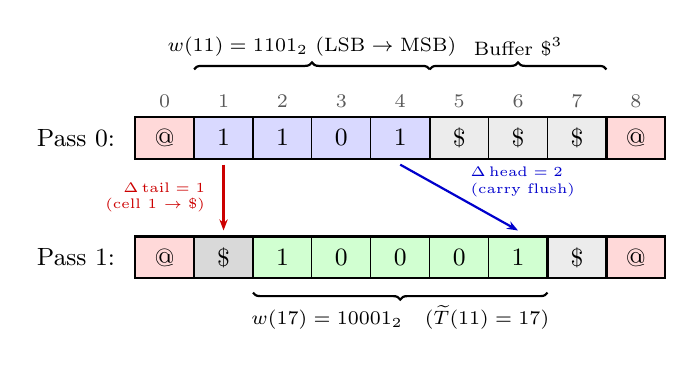
\begin{tikzpicture}[xscale=0.88, yscale=0.76]
% --- Top Brackets & Coordinate Labels ---
\draw[thick, decoration={brace, raise=2pt}, decorate] (0.85, 4.5) -- (4.25, 4.5)
    node[midway, above=3pt, font=\scriptsize] {$w(11) = 1101_2 \ (\text{LSB}\to\text{MSB})$};
\draw[thick, decoration={brace, raise=2pt}, decorate] (4.25, 4.5) -- (6.80, 4.5)
    node[midway, above=3pt, font=\scriptsize] {Buffer $\$^3$};

\foreach \x in {0,...,8} {
    \node[above, font=\scriptsize, text=gray!70!black] at (\x*0.85+0.425, 3.8) {\x};
}

% --- Pass 0 Cells (y: 3.1 to 3.8) ---
\draw[thick, fill=red!15] (0, 3.1) rectangle ++(0.85, 0.7) node[midway] {\small $@$};
\draw[thick, fill=blue!15] (0.85, 3.1) rectangle ++(3.4, 0.7);
\foreach \i/\b in {0/1, 1/1, 2/0, 3/1} {
    \draw (0.85+\i*0.85, 3.1) -- (0.85+\i*0.85, 3.8);
    \node at (0.85+\i*0.85+0.425, 3.45) {\small \b};
}
\draw[thick, fill=gray!15] (4.25, 3.1) rectangle ++(2.55, 0.7);
\foreach \i in {0,1,2} {
    \draw (4.25+\i*0.85, 3.1) -- (4.25+\i*0.85, 3.8);
    \node at (4.25+\i*0.85+0.425, 3.45) {\small $\$$};
}
\draw[thick, fill=red!15] (6.80, 3.1) rectangle ++(0.85, 0.7) node[midway] {\small $@$};
\node[left, font=\small] at (-0.15, 3.45) {Pass $0$:};

% --- Intermediate Transition Arrows (y: 1.8 to 3.1) ---
% Tail shift arrow at Cell 1 (x = 1.275)
\draw[-{Stealth[length=4pt]}, thick, red!80!black] (1.275, 3.0) -- (1.275, 1.9)
    node[midway, left=3pt, font=\tiny, text=red!80!black, align=right] {$\Delta\tail = 1$\\(cell 1 $\to \$$)};

% Head expansion arrow from Cell 4 to Cell 6 (x = 3.825 down to 5.525)
\draw[-{Stealth[length=4pt]}, thick, blue!80!black] (3.825, 3.0) -- (5.525, 1.9);
\node[font=\tiny, text=blue!80!black, align=left, anchor=south west] at (4.7, 2.3) {$\Delta\head = 2$\\(carry flush)};

% --- Pass 1 Cells (y: 1.1 to 1.8) ---
\draw[thick, fill=red!15] (0, 1.1) rectangle ++(0.85, 0.7) node[midway] {\small $@$};
\draw[thick, fill=gray!30] (0.85, 1.1) rectangle ++(0.85, 0.7) node[midway] {\small $\$$};
\draw[thick, fill=green!18] (1.70, 1.1) rectangle ++(4.25, 0.7);
\foreach \i/\b in {0/1, 1/0, 2/0, 3/0, 4/1} {
    \draw (1.70+\i*0.85, 1.1) -- (1.70+\i*0.85, 1.8);
    \node at (1.70+\i*0.85+0.425, 1.45) {\small \b};
}
\draw[thick, fill=gray!15] (5.95, 1.1) rectangle ++(0.85, 0.7) node[midway] {\small $\$$};
\draw[thick, fill=red!15] (6.80, 1.1) rectangle ++(0.85, 0.7) node[midway] {\small $@$};
\node[left, font=\small] at (-0.15, 1.45) {Pass $1$:};

% --- Bottom Bracket ---
\draw[thick, decoration={brace, mirror, raise=3pt}, decorate] (1.70, 1.0) -- (5.95, 1.0)
    node[midway, below=4pt, font=\scriptsize] {$w(17) = 10001_2 \quad (\widetilde{T}(11) = 17)$};
\end{tikzpicture}
\caption{Single-word tape cell coordinates and bit-serial execution of $\mathcal{M}'$ for $N=11$ ($1101_2 \to 10001_2 = 17$). Left-hand sentinel $@$ remains stationary at cell 0. Blank $\$$ overwrites the consumed LSB at cell 1 (on-the-fly $/2$ odd-core reduction, $\Delta\tail=1$). Carries propagate rightward (RHS = MSB) into the $\$$ buffer, advancing $\head$ by $\Delta\head=2$.}
\label{fig:tape_trace}
\end{figure}

\subsection{Operational Mechanics}
A cyclic four-phase sequence is executed autonomously across each pass $t$, as illustrated in Fig.~\ref{fig:tape_trace}:
\begin{enumerate}
    \item \textbf{Trailing Zero Elimination and LSB Detection (State $A$)}: Moving rightward across leading zeros, State $A$ writes blanks $\$$. Upon reading the odd-core LSB $1$, it writes $\$$ and transitions to State $B$.
    \item \textbf{Streaming Addition (States $B, C, D$)}: States $B$ and $C$ compute the bit-serial addition of $x + 2x + 1$ with carry states $c_{\text{in}} \in \{0, 1\}$. State $D$ handles internal zero propagation.
    \item \textbf{Self-Clearing Carry Flush}: At delimiter $\$$, the terminal carry bits are flushed: $B \xrightarrow{\$} (0, R, C) \xrightarrow{\$} (1, R, A)$. The carry is discharged within two cells, returning to State $A$ to process $N_{i+1}$ without tape reversal.
    \item \textbf{Autonomous Boundary Reflection and Rewind (States $A, E$)}: Upon encountering sentinel $@$ at the right horizon, $\delta(A, @) = (@, L, E)$ initiates leftward rewind. State $E$ traverses data and delimiters non-destructively. At cell 0 ($@$), $\delta(E, @) = (@, R, A)$ reflects the head into State $A$ for the next pass.
\end{enumerate}

\section{Spatial Drift and Collision Mechanics}

\subsection{Head and Tail Displacement}
For any number $N$ at pass $t$, let $\tail(N, t) \in \mathbb{N}$ denote the coordinate of the least significant bit, and $\head(N, t) \in \mathbb{N}$ denote the coordinate of the most significant bit.

\begin{lemma}[Displacement Bounds]
For any positive odd integer $N$ at pass $t \ge 0$ with 2-adic valuation $k_t = \nu_2(3 \cdot \oddcore(N) + 1) \ge 1$:
\begin{align}
\Delta \head(N, t) &= \head(N, t+1) - \head(N, t) \le 2 \label{eq:head_disp} \\
\Delta \tail(N, 0) &= 1 \label{eq:tail_disp_0} \\
\Delta \tail(N, t) &= \max\{1, k_{t-1}\} \quad \forall t \ge 1 \label{eq:tail_disp_t}
\end{align}
Specifically, $\Delta \tail(N, t) = 1$ when $T^{t-1}(N) \equiv 3 \pmod 4$ ($k_{t-1} = 1$), and $\Delta \tail(N, t) = k_{t-1} \ge 2$ when $T^{t-1}(N) \equiv 1 \pmod 4$ ($k_{t-1} \ge 2$).
\end{lemma}
\begin{proof}
At $t=0$, $N$ contains no leading zeros ($b_0 = 1$); State $A$ consumes only LSB $1$, giving $\Delta \tail = 1$. For $t \ge 1$, the adder divides by 2 on-the-fly, writing exactly $k_{t-1} - 1$ trailing zeros to tape. On pass $t$, State $A$ consumes these $k_{t-1}-1$ zeros plus the odd-core bit $1$. If $k_{t-1} = 1$, zero trailing zeros exist, yielding $\Delta \tail = 1$. If $k_{t-1} \ge 2$, $(k_{t-1}-1)+1 = k_{t-1} \ge 2$ cells are consumed. Concurrently, because $\widetilde{T}(m) = (3m+1)/2 \le 2m$ for all odd $m \ge 1$ (with strict inequality for $m > 1$ and equality for $m=1$), the bit-serial output length satisfies $L(\widetilde{T}(m)) - L(m) \le 1$. Since the adder begins writing at $\tail + 1$, the advance of the most significant bit is strictly bounded by $\Delta \head = 1 + (L(\widetilde{T}(m)) - L(m)) \le 2$ universally.
\end{proof}

\subsection{The Inter-Word Squeeze Phenomenon}
Consider two adjacent words $N_{x-1}$ and $N_x$ separated by instantaneous gap $\gap_t = \tail(N_x, t) - \head(N_{x-1}, t) - 1$. The change in spatial buffer per pass is governed by the 1D spatial recurrence (illustrated in Fig.~\ref{fig:drift_mechanics}):
\begin{equation}
\Delta \gap_t = \Delta \tail(N_x, t) - \Delta \head(N_{x-1}, t)
\label{eq:gap_evolution}
\end{equation}

\begin{proposition}[Initial Buffer Compression Under Ascent]
On pass $t = 0$, if $N_{x-1}$ undergoes maximum bit growth with $\Delta \head(N_{x-1}, 0) = 2$, while $N_x$ shifts by $\Delta \tail(N_x, 0) = 1$, the inter-word buffer compresses by $\Delta \gap_0 = 1 - 2 = -1$.
Consequently, initial spacing $S \ge 3$ is strictly required to guarantee $\gap_1 \ge 2$ on the first pass.
\end{proposition}

\begin{figure}[htbp]
\centering
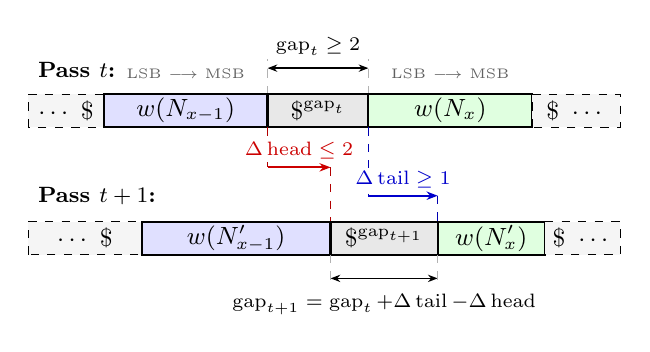
\begin{tikzpicture}[x=0.80cm, y=0.60cm]
% ===================== PASS t =====================
% Row title placed above tape row at top-left
\node[anchor=south west, font=\bfseries\footnotesize] at (0, 4.15) {Pass $t$:};

% Direction / Bit orientation labels above words
\node[above=2pt, font=\tiny, text=gray!75!black] at (2.5, 4.0) {LSB $\longrightarrow$ MSB};
\node[above=2pt, font=\tiny, text=gray!75!black] at (6.7, 4.0) {LSB $\longrightarrow$ MSB};

% Dimension line for gap_t above buffer cell
\draw[{Stealth[length=3.5pt]}-{Stealth[length=3.5pt]}, semithick] (3.8, 4.55) -- (5.4, 4.55)
    node[midway, above=1pt, font=\scriptsize] {$\gap_t \ge 2$};
\draw[dashed, gray!60] (3.8, 4.0) -- (3.8, 4.75);
\draw[dashed, gray!60] (5.4, 4.0) -- (5.4, 4.75);

% Cells for Pass t: total span x = 0 to 9.4, y in [3.3, 4.0]
\draw[dashed, fill=gray!8] (0, 3.3) rectangle (1.2, 4.0);
\node at (0.6, 3.65) {\small $\cdots\ \$$};

\draw[thick, fill=blue!12] (1.2, 3.3) rectangle (3.8, 4.0);
\node at (2.5, 3.65) {\small $w(N_{x-1})$};

\draw[thick, fill=gray!18] (3.8, 3.3) rectangle (5.4, 4.0);
\node at (4.6, 3.65) {\small $\$^{\gap_t}$};

\draw[thick, fill=green!12] (5.4, 3.3) rectangle (8.0, 4.0);
\node at (6.7, 3.65) {\small $w(N_x)$};

\draw[dashed, fill=gray!8] (8.0, 3.3) rectangle (9.4, 4.0);
\node at (8.7, 3.65) {\small $\$ \ \cdots$};

% ===================== INTER-PASS DYNAMICS =====================
% Red: Head expansion of Word N_{x-1} (upper tier at y = 2.45)
\draw[dashed, red!70!black] (3.8, 3.3) -- (3.8, 2.45);
\draw[-{Stealth[length=4pt]}, thick, red!80!black] (3.8, 2.45) -- (4.8, 2.45)
    node[midway, above=1.5pt, font=\scriptsize, text=red!80!black, fill=white, inner sep=1pt] {$\Delta\head \le 2$};
\draw[dashed, red!70!black] (4.8, 2.45) -- (4.8, 1.3);

% Blue: Tail shift of Word N_x (lower tier at y = 1.85)
\draw[dashed, blue!70!black] (5.4, 3.3) -- (5.4, 1.85);
\draw[-{Stealth[length=4pt]}, thick, blue!80!black] (5.4, 1.85) -- (6.5, 1.85)
    node[midway, above=1.5pt, font=\scriptsize, text=blue!80!black, fill=white, inner sep=1pt] {$\Delta\tail \ge 1$};
\draw[dashed, blue!70!black] (6.5, 1.85) -- (6.5, 1.3);

% ===================== PASS t+1 =====================
% Row title placed above tape row at top-left
\node[anchor=south west, font=\bfseries\footnotesize] at (0, 1.45) {Pass $t+1$:};

% Cells for Pass t+1: total span x = 0 to 9.4, y in [0.6, 1.3]
\draw[dashed, fill=gray!8] (0, 0.6) rectangle (1.8, 1.3);
\node at (0.9, 0.95) {\small $\cdots\ \$$};

\draw[thick, fill=blue!12] (1.8, 0.6) rectangle (4.8, 1.3);
\node at (3.3, 0.95) {\small $w(N'_{x-1})$};

\draw[thick, fill=gray!18] (4.8, 0.6) rectangle (6.5, 1.3);
\node at (5.65, 0.95) {\small $\$^{\gap_{t+1}}$};

\draw[thick, fill=green!12] (6.5, 0.6) rectangle (8.2, 1.3);
\node at (7.35, 0.95) {\small $w(N'_x)$};

\draw[dashed, fill=gray!8] (8.2, 0.6) rectangle (9.4, 1.3);
\node at (8.8, 0.95) {\small $\$ \ \cdots$};

% Dimension line for gap_{t+1} & recurrence below Pass t+1
\draw[{Stealth[length=3.5pt]}-{Stealth[length=3.5pt]}, semithick] (4.8, 0.10) -- (6.5, 0.10);
\node[below=2pt, font=\scriptsize] at (5.65, 0.10) {$\gap_{t+1} = \gap_t + \Delta\tail - \Delta\head$};
\draw[dashed, gray!60] (4.8, 0.6) -- (4.8, -0.10);
\draw[dashed, gray!60] (6.5, 0.6) -- (6.5, -0.10);
\end{tikzpicture}
\caption{Space-time inter-word displacement mechanics under $\mathcal{M}'$. In vector mode, inter-word coupling is fully governed by the single 1D spatial recurrence variable $\Delta \gap_t = \Delta\tail(N_x, t) - \Delta\head(N_{x-1}, t)$. Maintaining $\gap_t \ge 2$ preserves complete scalar operational equivalence for each word across the pipeline.}
\label{fig:drift_mechanics}
\end{figure}

\section{Non-Colliding Tape Architectures}

\subsection{Regime I: Sufficient Asymptotic Buffering}
In this regime, unconditional collision freedom is guaranteed through buffer sizing.

\begin{definition}[Cumulative Drift Differential]
Let $\mathcal{O}(N) = \{N, \widetilde{T}(N), \widetilde{T}^2(N), \dots\}$ denote the trajectory. The cumulative drift differential between words $N_i$ and $N_{i+1}$ is:
\begin{multline}
\mathcal{D}_{\max}(N_i, N_{i+1}) = \\
\max_{t \ge 0} \sum_{\tau=0}^t \big( \Delta \head(N_i, \tau) - \Delta \tail(N_{i+1}, \tau) \big)
\label{eq:dmax_def}
\end{multline}
\end{definition}

\begin{theorem}[Universal Collision Freedom Under Regime I]
Let the tape be $\mathcal{T}_0 = @ \, N_1 \, \$^{S_1} \dots \$^{S_{n-1}} \, N_n \, [\$] \, @^\omega$. If each initial inter-word buffer satisfies:
\begin{equation}
S_i \ge \mathcal{D}_{\max}(N_i, N_{i+1}) + 2
\label{eq:buffer_bound}
\end{equation}
then $\gap_t(N_i, N_{i+1}) \ge 2$ for all passes $t \ge 0$, guaranteeing that every word evaluates strictly independently into the right-infinite $@^\omega$ background without carry overrun.
\end{theorem}
\begin{proof}
By induction on pass index $t$. The instantaneous gap satisfies $\gap_t = S_i - \sum_{\tau=0}^{t-1} (\Delta \head_i - \Delta \tail_{i+1}) \ge S_i - \mathcal{D}_{\max}(N_i, N_{i+1})$. Under condition (\ref{eq:buffer_bound}), $\gap_t \ge 2$ holds for all $t \ge 0$. By Table~\ref{tab:transitions}, modifying writes of word $N_i$ during pass $t$ are strictly bounded by $\writemax(N_i, t) = \head(N_i, t) + 2$. Since $\tail(N_{i+1}, t) = \head(N_i, t) + 1 + \gap_t \ge \head(N_i, t) + 3$, we have $\writemax(N_i, t) < \tail(N_{i+1}, t)$ universally, preventing carry overrun into $N_{i+1}$.
\end{proof}

\subsection{Limits of Uniform Spacing: The Word-Length Invariant}
By Table~\ref{tab:transitions}, modifying writes of word $N_{x-1}$ are confined to $\writemax(N_{x-1}, t) = \head(N_{x-1}, t) + 2$.
When $\gap_t \ge 2$, safety invariant $\writemax(N_{x-1}, t) < \tail(N_x, t)$ holds strictly.

\begin{proposition}[Identical Trajectory Buffer Invariant]
\label{prop:identical_compression}
Let $N_{x-1} = N_x = N$ follow identical trajectories on tape. Since both words evaluate synchronously, their tail displacements are identical: $\Delta\tail(N_x, t) = \Delta\tail(N_{x-1}, t)$. Let $L(N, t) = \head(N, t) - \tail(N, t) + 1$ denote the physical binary word length on tape. Then:
\begin{equation}
\Delta\head(N_{x-1}, t) = \Delta\tail(N_{x-1}, t) + \Delta L(N, t)
\end{equation}
Consequently, the relative buffer evolution is governed entirely by word-length change:
\begin{equation}
\Delta\gap_t = \Delta\tail(N_x, t) - \Delta\head(N_{x-1}, t) = -\Delta L(N, t)
\label{eq:identical_gap_invariant}
\end{equation}
The inter-word buffer compresses by exactly the net bit growth of the word: $\gap_t = S - (L(N, t) - L(N, 0))$.
\end{proposition}
Whenever net word expansion satisfies $L(N, t) - L(N, 0) \ge S - 1$, uniform buffer $S$ inevitably collapses.
Conversely, for trajectories within the attractor, the word length is invariant ($L=2$, $\Delta L = 0$), yielding $\Delta \gap_t = 0$, where $S = 3$ remains unconditionally sufficient.

\section{Asymptotic Phase-Locking: Soliton Array Formation}
Under the Collatz conjecture, every odd integer reaches $1$ under $T(n)$ in finite stopping time $\sigma(N_i) < \infty$. Under the affine transducer operator $\widetilde{T}(n) = (3\oddcore(n)+1)/2$, $\widetilde{T}(1) = 2$ and $\widetilde{T}(2) = 2$. Thus, $N = 2$ is the unique singleton stationary fixed point of the operator $\widetilde{T}$.

\begin{definition}[Binary Limit Soliton]
In LSB binary representation, the fixed point $2$ corresponds to the binary word $\mathbf{s} = \texttt{01}_2$ (trailing zero followed by odd core $1$). The binary kernel $\mathbf{s} = \texttt{01}$ forms an invariant solitary wave packet on the tape.
\end{definition}

\begin{theorem}[Conditional Soliton Velocity and Spatial Freezing]
Assume Collatz convergence for $\mathbf{N} = \langle N_1, \dots, N_n \rangle$ with $t^* = \max_{1 \le i \le n} \sigma(N_i)$. For all passes $t \ge t^*$: (1)~every word reaches the stationary fixed point $N_i = 2$ ($\mathbf{s} = \texttt{01}$) propagating rightward at constant velocity $\vsoliton = 2$ cells/pass; (2)~inter-soliton distances freeze permanently with $\gap_t(N_i, N_{i+1}) = \text{const} \ge 2$; and (3)~the global tape converges to a phase-locked travelling soliton array:
\begin{equation}
\mathcal{T}_\infty = @ \, \$^{d_0} \, \mathbf{s} \, \$^{d_1} \, \mathbf{s} \, \$^{d_2} \dots \mathbf{s} \, @^\omega, \quad d_i \in \mathbb{N}_{\ge 2}
\label{eq:soliton_array}
\end{equation}
where each soliton translates rigidly at $v = 2$ cells/pass. While group velocity is uniform and relative distances freeze ($\Delta \gap_t = 0$), the array is generally spatially aperiodic, with frozen spacings $d_i$ determined by the initial vector $\mathbf{N}$ and transient stopping times $\sigma(N_i)$.
\end{theorem}
\begin{proof}
For the soliton kernel $\mathbf{s} = \texttt{01}$ ($N=2$), the word occupies two cells: trailing zero $\texttt{0}$ at coordinate $\tail$ and odd-core bit $\texttt{1}$ at coordinate $\tail+1$. On each pass, State $A$ consumes the trailing zero ($\delta(A, 0) = (\$, R, A)$) and the odd-core bit ($\delta(A, 1) = (\$, R, B)$), shifting the tail by $\Delta\tail = 2$ cells. In State $B$, the adder computes the affine map $\widetilde{T}(2) = (3(1)+1)/2 = 2$: the carry flush across two delimiter cells $\$$ outputs $\texttt{0}$ ($\delta(B, \$) = (0, R, C)$) and $\texttt{1}$ ($\delta(C, \$) = (1, R, A)$), shifting the head by $\Delta\head = 2$ cells and reconstructing $\mathbf{s} = \texttt{01}$ identically. Because $\Delta\tail = \Delta\head = 2$, each word preserves its bit length ($L = 2$) and translates rigidly by $v = 2$ cells per pass. The spatial gap velocity between adjacent words satisfies $\Delta\gap_t = \Delta\tail(N_{i+1}) - \Delta\head(N_i) = 2 - 2 = 0$, freezing the spatial configuration permanently.
\end{proof}

\section{Simulation and Empirical Verification}
The theoretical bounds were verified through discrete-event simulation using the Python verification harness \cite{varshney2026notes}.

\subsection{Buffer Collapse Case Study \texorpdfstring{($N_1 = 7, N_2 = 1, S = 2$)}{(N1=7, N2=1, S=2)}}
Evaluating $N_1 = 7$ (`\texttt{111}') and $N_2 = 1$ (`\texttt{1}') with insufficient buffer $S = 2$: at \textbf{Pass 1} ($7 \to 11$, $1 \to 2$), the buffer compresses from $2$ to $1$ cell: $\mathcal{T}_1 = \texttt{@ \$ 1101 \$ 01 @}$. At \textbf{Pass 2} ($11 \to 17$), the carry chain overruns the single $\$$ delimiter at step 23, reading the LSB of $N_2$ in State $C$ and overwriting it via $\delta(C, 0) = (1, R, D)$, fusing both words into $\texttt{100011}$.

\subsection{Counterexample Verification \texorpdfstring{($N_1 = 27, N_2 = 27, S = 3$)}{(N1=27, N2=27, S=3)}}
Evaluating $\mathbf{N} = \langle 27, 27 \rangle$ under $S = 3$: $27$ ascends through $\{41, 31, 47, 71, 107, 161\}$ with binary word lengths $L \in \{5, 6, 6, 6, 7, 7, 8\}$. By Proposition~\ref{prop:identical_compression}, identical trajectories satisfy $\Delta \gap_t = -\Delta L(N, t)$. Consequently, the buffer contracts with each bit growth: $\gap_0 = 3 \to 2 \to 2 \to 2 \to 1 \to 1 \to 0 = \gap_6$ under pass decrements $(-1, 0, 0, -1, 0, -1)$. At Pass 6, Word 1 overruns Word 2, producing $\texttt{@\$\$\$\$\$\$\$1000010010000101@}$ with zero separating blanks.

\subsection{Regime I Verification \texorpdfstring{($N_1 = 27, N_2 = 27, S = 15$)}{(N1=27, N2=27, S=15)}}
With buffer $S = 15 \ge \mathcal{D}_{\max}(27, 27) + 2 = 7$, $\gap_t$ remains strictly $\ge 10 \ge 2$ across all ascents. At Pass 8, both trajectories evaluate safely with complete isolation.

\section{Formal Lean 4 Certification}
\label{sec:lean_verification}
\begin{sloppypar}
All operational semantics, transition invariants, and collision-free drift mechanics of transducer $\mathcal{M}'$ have been machine-checked in Lean~4~\cite{moura2021} without auxiliary axioms or \texttt{sorry} gaps (pinned to \texttt{v4.14.0}, reproducible via \texttt{lake build}). The machine-checked corpus formally certifies:
(1)~\textbf{Transition Completeness}: exactly 18 active transitions over 20 domain cells (\texttt{active\_\allowbreak transitions\_\allowbreak eq\_\allowbreak eighteen});
(2)~\textbf{Displacement Bounds} (Lemma~1): tail shift $\Delta \tail(n, t) = \max\{1, k_{t-1}\}$ for all $k$ (\texttt{tail\_\allowbreak disp\_\allowbreak pos}, \texttt{tail\_\allowbreak disp\_\allowbreak eq\_\allowbreak one\_\allowbreak of\_\allowbreak k\_\allowbreak one}, \texttt{tail\_\allowbreak disp\_\allowbreak ge\_\allowbreak two\_\allowbreak of\_\allowbreak k\_\allowbreak ge\_\allowbreak two});
(3)~\textbf{Regime I Sufficiency} (Theorem~1): buffer preservation $\gap_t \ge 2$ under $S \ge \mathcal{D}_{\max} + 2$ and write-separation soundness (\texttt{regime\_\allowbreak I\_\allowbreak safe\_\allowbreak separation}, \texttt{write\_\allowbreak separation\_\allowbreak sound});
(4)~\textbf{Soliton Dynamics} (Theorem~2): rigid translation at group velocity $v = 2$ cells/pass and spatial gap velocity freezing (\texttt{soliton\_\allowbreak rigid\_\allowbreak translation}, \texttt{soliton\_\allowbreak gap\_\allowbreak freezing});
(5)~\textbf{Word-Length Invariant} (Proposition~\ref{prop:identical_compression}): $\Delta\gap_t = -\Delta L_t$ (\texttt{identical\_\allowbreak words\_\allowbreak gap\_\allowbreak compression}); and
(6)~\textbf{Preimage Inversion}: exact ancestor recovery $n = (m \cdot 2^k - 1)/3$ (\texttt{reverse\_\allowbreak exactness}).
The complete Lean formalization is archived in repository records~\cite{varshney2026notes}.
\end{sloppypar}

\section{Architectural Proposal: Reversible Inversion via Spatial Drift Decoupling}
\label{sec:reversible_drift}
While the scalar Syracuse operator $T(n) = (3n+1)/2^k$ is non-injective over odd integers, the augmented dynamical map $\Phi: 2\mathbb{N}+1 \longleftrightarrow \mathcal{S}_{\text{admit}}$, $n \mapsto (m, k)$ is a strict mathematical bijection, where $\mathcal{S}_{\text{admit}} = \{ (m, k) \in (2\mathbb{N}+1) \times \mathbb{N}_{\ge 1} : m \cdot 2^k \equiv 1 \pmod 3 \}$, with unique odd ancestor $n = (m \cdot 2^k - 1)/3$. Although transducer $\mathcal{M}'$ is forward-deterministic, trailing zeros are overwritten by anonymous blanks $\$$ in State $A$. The physical tail displacement satisfies $\Delta \tail(N, t) = \max\{1, k_{t-1}\}$. For the lead word $N_1$ adjacent to static sentinel $@$, absolute displacement from cell 0 uniquely records cumulative $\Delta\tail(N_1, t)$, preserving $k$ without ambiguity. For interior words $N_{x \ge 2}$, the delimiter gap $\gap_t = \tail(N_x, t) - \head(N_{x-1}, t) - 1$ records relative displacement $\Delta\tail(N_x, t) - \Delta\head(N_{x-1}, t)$, conflating the valuation of $N_x$ with the carry growth of $N_{x-1}$. Consequently, deterministic backward reconstruction requires sequential left-to-right uncoupling. A companion reversible transducer $\mathcal{M}_{\text{rev}}'$ anchored at $@$ must invert $N_1$ first, compute $\Delta\head(N_1, t)$, uncouple $\Delta\tail(N_2, t)$ from $\gap_t$, and cascade backward evaluation across the pipeline without auxiliary tape registers~\cite{yokoyama2020,fredkin1982}.

\section{Conclusion and Open Problems}
\label{sec:conclusion}
The formal mechanics of autonomous multi-trajectory Syracuse computation on small Turing transducers have been established. By identifying the exact conditions under which spatial drift preserves word isolation, Regime I buffer sizing ($S_i \ge \mathcal{D}_{\max} + 2$) was proven to unconditionally prevent carry overrun, while the exact failure boundary of uniform $O(1)$ spacing was delineated via bit-length growth ($\Delta\gap_t = -\Delta L_t$).
Two open problems emerge: (1)~\textbf{State Minimality}: proving whether 4 states are strictly insufficient for cyclic multi-trajectory Syracuse computation under equivalent alphabets; and (2)~\textbf{Reversible Automation}: formalizing the sequential uncoupling automaton $\mathcal{M}_{\text{rev}}'$ to invert the pipeline deterministically via spatial drift geometry. Future work will examine the embedding of these drift-dominant sequences into reversible cellular automata for the 19th International Conference on Reversible Computation (RC 2027)~\cite{wolfram2002}.

\begin{thebibliography}{10}
\bibitem{conway1972}
J.~H. Conway, ``Unpredictable iterations,'' in \emph{Proc. 1972 Number Theory Conf.}, Boulder, CO, 1972, pp. 49--52.

\bibitem{lagarias1985}
J.~C. Lagarias, ``The $3x + 1$ problem and its generalizations,'' \emph{Amer. Math. Monthly}, vol. 92, no. 1, pp. 3--23, 1985.

\bibitem{terras1976}
R.~Terras, ``A stopping time problem on the positive integers,'' \emph{Acta Arithmetica}, vol. 30, no. 3, pp. 241--252, 1976.

\bibitem{margenstern2000}
M.~Margenstern, ``Frontier between decidability and undecidability: A survey,'' \emph{Theor. Comput. Sci.}, vol. 231, no. 2, pp. 217--251, 2000.

\bibitem{woods2009}
D.~Woods and T.~Neary, ``The complexity of small universal Turing machines: A survey,'' \emph{Theor. Comput. Sci.}, vol. 410, no. 4-5, pp. 443--450, 2009.

\bibitem{baiocchi2001}
C.~Baiocchi, ``Collatz trajectories and cellular automata,'' \emph{Complex Systems}, vol. 13, no. 1, pp. 33--48, 2001.

\bibitem{michel2010}
P.~Michel and M.~Margenstern, ``Collatz trajectories and small Turing machines,'' in \emph{Proc. 6th MCU}, LNCS, vol. 6140, pp. 110--123, Springer, 2010.

\bibitem{fredkin1982}
E.~Fredkin and T.~Toffoli, ``Conservative logic,'' \emph{Int. J. Theor. Phys.}, vol. 21, no. 3-4, pp. 219--253, 1982.

\bibitem{yokoyama2020}
T.~Yokoyama, ``Reversible computation and reversible Turing machines,'' \emph{LNCS}, vol. 12227, pp. 3--18, Springer, 2020.

\bibitem{wolfram2002}
S.~Wolfram, \emph{A New Kind of Science}. Champaign, IL: Wolfram Media, 2002.

\bibitem{moura2021}
L.~de Moura and S.~Ullrich, ``The Lean 4 theorem prover and programming language,'' in \emph{Proc. CADE-28}, LNCS, vol. 12699, pp. 625--635, Springer, 2021.

\bibitem{varshney2026notes}
L.~Varshney, ``Autonomous Syracuse transducer verification suite and technical archive,'' Zenodo, Nov. 2026, doi: \href{https://doi.org/10.5281/zenodo.24223304}{10.5281/zenodo.24223304}.
\end{thebibliography}

\end{document}
